\documentclass[presentation,aspectratio=43, 10pt]{beamer}
\usepackage{pifont}
\newcommand{\cmark}{\ding{51}}
\newcommand{\xmark}{\ding{55}}
\usepackage{changepage}
\usepackage{booktabs}
\titlegraphic{\hfill
\includegraphics[height=1.25cm]{durham-logo}}
\usepackage{appendixnumberbeamer}
\def\xunderbrace#1_#2{{\underbrace{#1}_{\mathclap{#2}}}}
\def\xoverbrace#1^#2{{\overbrace{#1}^{\mathclap{#2}}}}
\def\xunderarrow#1_#2{{\underset{\overset{\uparrow}{\mathclap{#2}}}{#1}}}
\def\xoverarrow#1^#2{{\overset{\underset{\downarrow}{\mathclap{#2}}}{#1}}}
\usepackage{amsmath}
\usepackage{amssymb}
\usepackage{mathtools}
\usepackage{hyperref}
\usepackage{xspace}
\newcommand{\arxivlink}[2]{{\texttt{arXiv:\,\href{https://arxiv.org/abs/#1}{#1\,[#2]}}}}
\usepackage{standalone}

\newcommand{\honev}{\ensuremath{{H}^1(\Omega; \mathbb{R}^d)}\xspace}
\newcommand{\ltwov}{\ensuremath{{L}^2(\Omega; \mathbb{R}^d)}\xspace}
\newcommand{\ltwo}{\ensuremath{{L}^2(\Omega)}\xspace}
\newcommand{\inner}[1]{\left\langle #1 \right \rangle}
\newcommand{\dx}{\ \text{d}x}
\setbeamersize{text margin left=0.5cm, text margin right=0.5cm}
\usepackage{minted}
\usepackage[url=false,
doi=true,
isbn=false,
style=authoryear,
maxnames=5,
giveninits=true,
uniquename=false,
backend=biber]{biblatex}
\renewcommand{\bibfont}{\fontsize{7}{7}\selectfont}
\addbibresource{references.bib}
\setbeamertemplate{bibliography item}[triangle]
\defbibenvironment{bibliography}
  {\list{}
     {\settowidth{\labelwidth}{\usebeamertemplate{bibliography item}}%
      \setlength{\leftmargin}{\labelwidth}%
      \setlength{\rightmargin}{\labelwidth}%
      \setlength{\labelsep}{\biblabelsep}%
      \addtolength{\leftmargin}{\labelsep}%
      \setlength{\itemsep}{\bibitemsep}%
      \setlength{\parsep}{\bibparsep}}}
  {\endlist}
  {\item}
\setlength{\bibitemsep}{1ex}
\setlength{\fboxsep}{1pt}

\renewbibmacro{in:}{}
\DeclareFieldFormat[article]{volume}{\textbf{#1}}
\DeclareFieldFormat{doi}{%
  doi\addcolon%
  {\scriptsize\ifhyperref{\href{http://dx.doi.org/#1}{\nolinkurl{#1}}}
    {\nolinkurl{#1}}}}
\AtEveryBibitem{%
\clearfield{pages}%
\clearfield{issue}%
\clearfield{number}%
}

\DeclareMathOperator{\grad}{grad}
\let\div\relax
\DeclareMathOperator{\div}{div}
\DeclareMathOperator{\curl}{curl}
\DeclareMathOperator{\range}{range}
\DeclareMathOperator{\sym}{sym}
\usetheme{metropolis}
\setbeamertemplate{title graphic}{
  \vbox to 0pt {
    \vspace*{1em}
    \inserttitlegraphic%
  }%
  \nointerlineskip%
}
\metroset{background=light,progressbar=frametitle,numbering=counter,block=fill}

% https://www.dur.ac.uk/marketingandcommunications/marketing/branding/colourpalette/
% Most of these are indistinguishable to those suffering colour blindness
\definecolor{purple}{HTML}{68246D}
\definecolor{blue}{HTML}{002A41}
\definecolor{red}{HTML}{BE1E2D}
\definecolor{cyan}{HTML}{00AEEF}
\definecolor{yellow}{HTML}{FFD53A}
\definecolor{green}{HTML}{00D53A}

\newenvironment{variableblock}[3]
{\setbeamercolor{block body}{#2}
\setbeamercolor{block title}{#3}
\begin{block}{#1}}%
{\end{block}}
  
\newenvironment{challenge}[1]%
{\begin{variableblock}{#1}{bg=red!20,fg=black}{bg=red,fg=white}}%
{\end{variableblock}}

\newenvironment{answer}[1]%
{\begin{variableblock}{#1}{bg=cyan!20,fg=black}{bg=cyan,fg=white}}%
{\end{variableblock}}

\renewenvironment{exampleblock}[1]%
{\begin{variableblock}{#1}{bg=yellow!20,fg=black}{bg=yellow,fg=white}}%
{\end{variableblock}}

\newcommand{\advect}[2]{\ensuremath{(#2 \cdot \nabla) #1}}
\newcommand{\kerdiv}{\ker\div}
\newcommand{\kercurl}{\ker\curl}
\let\Re\relax
\DeclareMathOperator{\Re}{Re}

\setbeamercolor{normal text}{
  fg=black,
  bg=white
}
\setbeamercolor{alerted text}{
  fg=red
}
\setbeamercolor{example text}{
  fg=blue
}

\setbeamercolor{palette primary}{%
  use=normal text,
  fg=normal text.bg,
  bg=purple,
}

\usetheme{metropolis}

\author{Lawrence Mitchell\inst{1,*} \\
  \and {\scriptsize
    P.~E.~Farrell (Oxford)
    \and
    L.~R.~Scott (Chicago)
    \and
    F.~Wechsung (Oxford)}}
\institute{
  \inst{1}Department of Computer Science, Durham University\\
  \inst{*}\texttt{lawrence.mitchell@durham.ac.uk}}

\title{A robust preconditioner for the stationary incompressible
  Navier--Stokes equations}

\usepackage{tikz}
\usetikzlibrary{trees,calc,positioning, trees}
\usetikzlibrary{shapes, shapes.geometric}
\usetikzlibrary{arrows,chains,positioning,fit,backgrounds,calc,shapes,
  shadows,scopes,decorations.markings,plotmarks}

\usepackage{expl3}

\ExplSyntaxOn
\newcommand{\fpeval}[1]{\fp_eval:n{#1}}
\ExplSyntaxOff

\newcommand{\DrawIterated}[7]% number of iterations
{ \ifnum#1=1%
  \draw[line join=round] (#2,#3) -- (#4,#5) -- (#6,#7) -- cycle;
  \else
  \draw[line join=round] (#2,#3) -- (#4,#5) -- (#6,#7) -- cycle;
  % Middle
  \DrawIterated{\numexpr#1-1\relax}%
  {\fpeval{(#2 + #4)/2}}%
  {\fpeval{(#3 + #5)/2}}%
  {\fpeval{(#4 + #6)/2}}%
  {\fpeval{(#5 + #7)/2}}%
  {\fpeval{(#2 + #6)/2}}%
  {\fpeval{(#3 + #7)/2}}

  % Bottom left
  \DrawIterated{\numexpr#1-1\relax}%
  {#2}%
  {#3}%
  {\fpeval{(#2 + #4)/2}}%
  {\fpeval{(#3 + #5)/2}}%
  {\fpeval{(#2 + #6)/2}}%
  {\fpeval{(#3 + #7)/2}}

  % Bottom right
  \DrawIterated{\numexpr#1-1\relax}%
  {\fpeval{(#2 + #4)/2}}%
  {\fpeval{(#3 + #5)/2}}%
  {#4}%
  {#5}%
  {\fpeval{(#4 + #6)/2}}%
  {\fpeval{(#5 + #7)/2}}%

  % Top
  \DrawIterated{\numexpr#1-1\relax}%
  {\fpeval{(#2 + #6)/2}}%
  {\fpeval{(#3 + #7)/2}}
  {\fpeval{(#4 + #6)/2}}%
  {\fpeval{(#5 + #7)/2}}%
  {#6}%
  {#7}
  
  \fi
}

\newcommand{\DrawIteratedBary}[7]% number of iterations
{ \ifnum#1=1%
  \draw[line join=round] (#2,#3) -- (#4,#5) -- (#6,#7) -- cycle;
  \coordinate (0) at (#2,#3);
  \coordinate (1) at (#4,#5);
  \coordinate (2) at (#6,#7);
  \coordinate (bc) at (barycentric cs:0=1,1=1,2=1);
  \draw[line join=round] (0) -- (bc) -- (1) (bc) -- (2);
  \else
  \draw[line join=round] (#2,#3) -- (#4,#5) -- (#6,#7) -- cycle;
  % Middle
  \DrawIteratedBary{\numexpr#1-1\relax}%
  {\fpeval{(#2 + #4)/2}}%
  {\fpeval{(#3 + #5)/2}}%
  {\fpeval{(#4 + #6)/2}}%
  {\fpeval{(#5 + #7)/2}}%
  {\fpeval{(#2 + #6)/2}}%
  {\fpeval{(#3 + #7)/2}}

  % Bottom left
  \DrawIteratedBary{\numexpr#1-1\relax}%
  {#2}%
  {#3}%
  {\fpeval{(#2 + #4)/2}}%
  {\fpeval{(#3 + #5)/2}}%
  {\fpeval{(#2 + #6)/2}}%
  {\fpeval{(#3 + #7)/2}}

  % Bottom right
  \DrawIteratedBary{\numexpr#1-1\relax}%
  {\fpeval{(#2 + #4)/2}}%
  {\fpeval{(#3 + #5)/2}}%
  {#4}%
  {#5}%
  {\fpeval{(#4 + #6)/2}}%
  {\fpeval{(#5 + #7)/2}}%

  % Top
  \DrawIteratedBary{\numexpr#1-1\relax}%
  {\fpeval{(#2 + #6)/2}}%
  {\fpeval{(#3 + #7)/2}}
  {\fpeval{(#4 + #6)/2}}%
  {\fpeval{(#5 + #7)/2}}%
  {#6}%
  {#7}
  
  \fi
}

\newcommand*{\tettextsize}{\footnotesize}
\tikzstyle{line} = [draw, -, thick]
\tikzstyle{nodraw} = [draw, fill, circle, minimum width=0pt, inner sep=0pt]
\tikzstyle{sieve} = [line, circle, font=\tettextsize, inner sep=0pt,
  minimum size=12pt]

\tikzstyle{cell} = [sieve, fill=blue!60]
\tikzstyle{facet} = [sieve, fill=green!35]
\tikzstyle{edge} = [sieve, fill=red!35]
\tikzstyle{vertex} = [sieve, fill=blue!35]

% https://tex.stackexchange.com/questions/27171/padded-boundary-of-convex-hull
\newcommand{\convexpath}[2]{
  [
  create hullcoords/.code={
    \global\edef\namelist{#1}
    \foreach [count=\counter] \nodename in \namelist {
      \global\edef\numberofnodes{\counter}
      \coordinate (hullcoord\counter) at (\nodename);
    }
    \coordinate (hullcoord0) at (hullcoord\numberofnodes);
    \pgfmathtruncatemacro\lastnumber{\numberofnodes+1}
    \coordinate (hullcoord\lastnumber) at (hullcoord1);
  },
  create hullcoords
  ]
  ($(hullcoord1)!#2!-90:(hullcoord0)$)
  \foreach [
  evaluate=\currentnode as \previousnode using \currentnode-1,
  evaluate=\currentnode as \nextnode using \currentnode+1
  ] \currentnode in {1,...,\numberofnodes} {
    let \p1 = ($(hullcoord\currentnode) - (hullcoord\previousnode)$),
    \n1 = {atan2(\y1,\x1) + 90},
    \p2 = ($(hullcoord\nextnode) - (hullcoord\currentnode)$),
    \n2 = {atan2(\y2,\x2) + 90},
    \n{delta} = {Mod(\n2-\n1,360) - 360}
    in
    {arc [start angle=\n1, delta angle=\n{delta}, radius=#2]}
    -- ($(hullcoord\nextnode)!#2!-90:(hullcoord\currentnode)$)
  }
}

\usepackage{pgfplots}
\pgfplotsset{compat=1.16}
\usetikzlibrary{plotmarks}
\usepackage{pgfplotstable}

\graphicspath{{./\jobname.figures/}{../pictures/}}
\date{10 June 2019}

\begin{document}

\maketitle

% \begin{abstract}
%   The Navier--Stokes equations are of enormous practical importance in
%   science and industry, but are notoriously difficult to solve,
%   especially for large Reynolds number.

%   In this talk, I will present a scalable multilevel preconditioner
%   for the stationary incompressible form of these equations which
%   exhibits iteration counts almost independent of the Reynolds number
%   and mesh resolution.

%   The implementation relies on a multigrid small patch additive
%   overlapping Schwarz smoother, and I will describe the computational,
%   and numerical analysis challenges in designing a robust choice.

%   I will present results using the Firedrake finite element library
%   solving problems with up to a billion degrees of freedom, and
%   describe some of the general preconditioning features that are now
%   available in Firedrake as a result of this work.

%   This is joint work with Patrick Farrell and Florian Wechsung
%   (Oxford), and Ridg Scott (Chicago).
% \end{abstract}



\begin{frame}[t]
  \frametitle{Setting}

  \begin{columns}
    \begin{column}{0.8\textwidth}
      \begin{quote}
        Firedrake \url{www.firedrakeproject.org} {\normalfont
          [\ldots]} is an automated system for the solution of
        partial differential equations using the finite element
        method.
      \end{quote}
    \end{column}
    \begin{column}{0.2\textwidth}
      
\includegraphics[width=0.8\textwidth]{firedrake-small}
    \end{column}
  \end{columns}
  \begin{itemize}
  \item Finite element problems specified with \emph{embedded}
    domain specific language, UFL \parencite{Alnaes:2014} from the
    FEniCS project.
  \item \emph{Runtime} compilation to optimised, low-level (C)
    code.
  \item PETSc for meshes and (algebraic) solvers.\par
    {\hfill \raggedleft \scriptsize \textcite{Rathgeber:2016} \arxivlink{1501.01809}{cs.MS}}
  \end{itemize}

  \begin{challenge}{Advert}
    3rd Firedrake user meeting is in Durham 26 \& 27 September 2019.

    {\centering \url{www.firedrakeproject.org/firedrake_19.html}\par}
    
  \end{challenge}
\end{frame}



\begin{frame}
  \frametitle{The problem}
  \begin{block}{Stationary, Newtonian, incompressible Navier--Stokes}
    Find $(u, p) \in \honev \times \ltwo$ such that
    \begin{alignat*}{2}
      -  \nu \nabla^2 u + \advect{u}{u} + \nabla p &= f \quad && \text{ in } \Omega, \\
      \nabla \cdot u &= 0 \quad && \text{ in } \Omega,
    \end{alignat*}
    with suitable boundary conditions, and $\nu$ the kinematic viscosity.
  \end{block}
  \begin{exampleblock}{Multiple solutions}<2->
    For $\nu \to 0$, these equations admit multiple solutions
  \end{exampleblock}
  \begin{challenge}{Motivating question}<3->
    What are the solution(s) as $\nu$ varies?
  \end{challenge}
\end{frame}

\begin{frame}
  \frametitle{Solving for the Newton step}
  \begin{block}{Newton linearisation}
    \begin{alignat*}{2}
      - \nu \nabla^2 u + \advect{w}{u} + \advect{u}{w} +
      \nabla p &= f \quad && \text{ in } \Omega, \\
      \nabla \cdot u &= 0 \quad && \text { in } \Omega.
    \end{alignat*}
  \end{block}
  \begin{columns}[t]
    \begin{column}{0.48\textwidth}
      \begin{block}{LU factorisation}
        \begin{itemize}
        \item[\cmark] Scales well with $\nu \to 0$
        \item[\xmark] Scales poorly with dof count
        \end{itemize}
      \end{block}
    \end{column}
    \begin{column}{0.48\textwidth}
      \begin{block}{Existing preconditioners}
        \begin{itemize}
        \item[\xmark] Convergence degrades with $\nu \to 0$
        \item[\cmark] Scales well with dof count
        \end{itemize}
      \end{block}
    \end{column}
  \end{columns}
  \begin{answer}{This talk}
    First preconditioner to scale well with $\nu$ and dof count in 3D.
  \end{answer}
\end{frame}

\section{Block preconditioners}
\begin{frame}
  \frametitle{Stokes}
  \begin{block}{Stokes' equations}
    Find $(u, p) \in H^1(\Omega)^d \times L^2(\Omega)$ such that
    \begin{alignat*}{2}
      -  \nu \nabla^2 u + \nabla p &= f \quad && \text{ in } \Omega, \\
      \nabla \cdot u &= 0 \quad && \text{ in } \Omega, \\
    \end{alignat*}
  \end{block}
  \begin{exampleblock}{Discretisation}
    Choosing an inf-sup stable element pair yields
    \begin{equation*}
      \mathcal{J}x := \begin{pmatrix}
        A & B^T \\
        B & 0
      \end{pmatrix}
      \begin{pmatrix}
        u \\ p
      \end{pmatrix}
      =
      \begin{pmatrix}
        f \\ 0
      \end{pmatrix}.
    \end{equation*}
  \end{exampleblock}
\end{frame}

\begin{frame}
  \frametitle{Preconditioners for block matrices}
  \begin{block}{Block factorisation \parencite{Murphy:2000}}
    Build preconditioners based on
    \begin{equation*}
      \mathcal{J}^{-1} = \begin{pmatrix}
        I & -A^{-1}B^T \\
        0 & I
      \end{pmatrix}
      \begin{pmatrix}
        A^{-1} & 0 \\
        0 & S^{-1}
      \end{pmatrix}
      \begin{pmatrix}
        I & 0 \\
        - BA^{-1} & I 
      \end{pmatrix}
    \end{equation*}
    where $S$ is the (usually dense!) Schur complement
    \begin{equation*}
      S = -BA^{-1} B^T.
    \end{equation*}
  \end{block}
  \pause
  \begin{challenge}{PDE-specific challenges}
    Find cheap, fast, approximations $\tilde{A}^{-1}$ and
    $\tilde{S}^{-1}$ to $A^{-1}$ and $S^{-1}$.
  \end{challenge}
\end{frame}

\begin{frame}
  \frametitle{Choosing $\tilde{A}^{-1}$ and $\tilde{S}^{-1}$}
  \begin{exampleblock}{Stokes \parencite{Silvester:1994}}
    Multigrid for $\tilde{A}^{-1}$, and choose $\tilde{S}^{-1} \sim
    M_p^{-1}$ ($M_p$ the pressure mass matrix).
  \end{exampleblock}
  \pause
  \begin{challenge}{Bad news}
    Mesh independent, but for \emph{Navier--Stokes}, choosing $\tilde{S}^{-1} \sim M_p^{-1}$
    degrades like $\mathcal{O}(\nu^{-2})$.
  \end{challenge}
  \pause
  \begin{answer}{PCD for Navier--Stokes \parencite{Kay:2002}}
    Approximate $S^{-1}$ with convection-diffusion solves on pressure
    space. Mesh independent, but degrades like
    $\mathcal{O}(\nu^{-1/2})$.
  \end{answer}
\end{frame}
\begin{frame}
  \frametitle{Performance of pressure convection-diffusion (PCD)}
\begin{table}[htbp]
\centering
\begin{tabular}{cc|c@{\hspace{9pt}}c@{\hspace{9pt}}c}
\toprule
$1/h$ & \# degrees of freedom & \multicolumn{3}{c}{Reynolds number} \\
  && 10 & 100 & 1000 \\
\midrule
$2^4$ & $8.34 \times 10^2$ & 22.0 & 40.4 & 103.3 \\
$2^5$ & $3.20 \times 10^3$ & 23.0 & 41.3 & 137.7 \\
$2^6$ & $1.25 \times 10^4$ & 24.5 & 42.0 & 157.0 \\
$2^7$ & $4.97 \times 10^4$ & 25.5 & 42.7 & 149.0 \\
$2^8$ & $1.98 \times 10^5$ & 26.0 & 44.0 & 137.0 \\
\bottomrule
\end{tabular}
\caption{Average number of outer Krylov iterations per Newton step for the
2D regularized lid-driven cavity problem with PCD preconditioner.
Obtained with IFISS v3.5, $Q_1-P_0$ element pair.}
\label{tab:pcdlscldc}
\end{table}
\end{frame}

\section{Augmented Lagrangian preconditioners}

\begin{frame}
  \begin{center}
    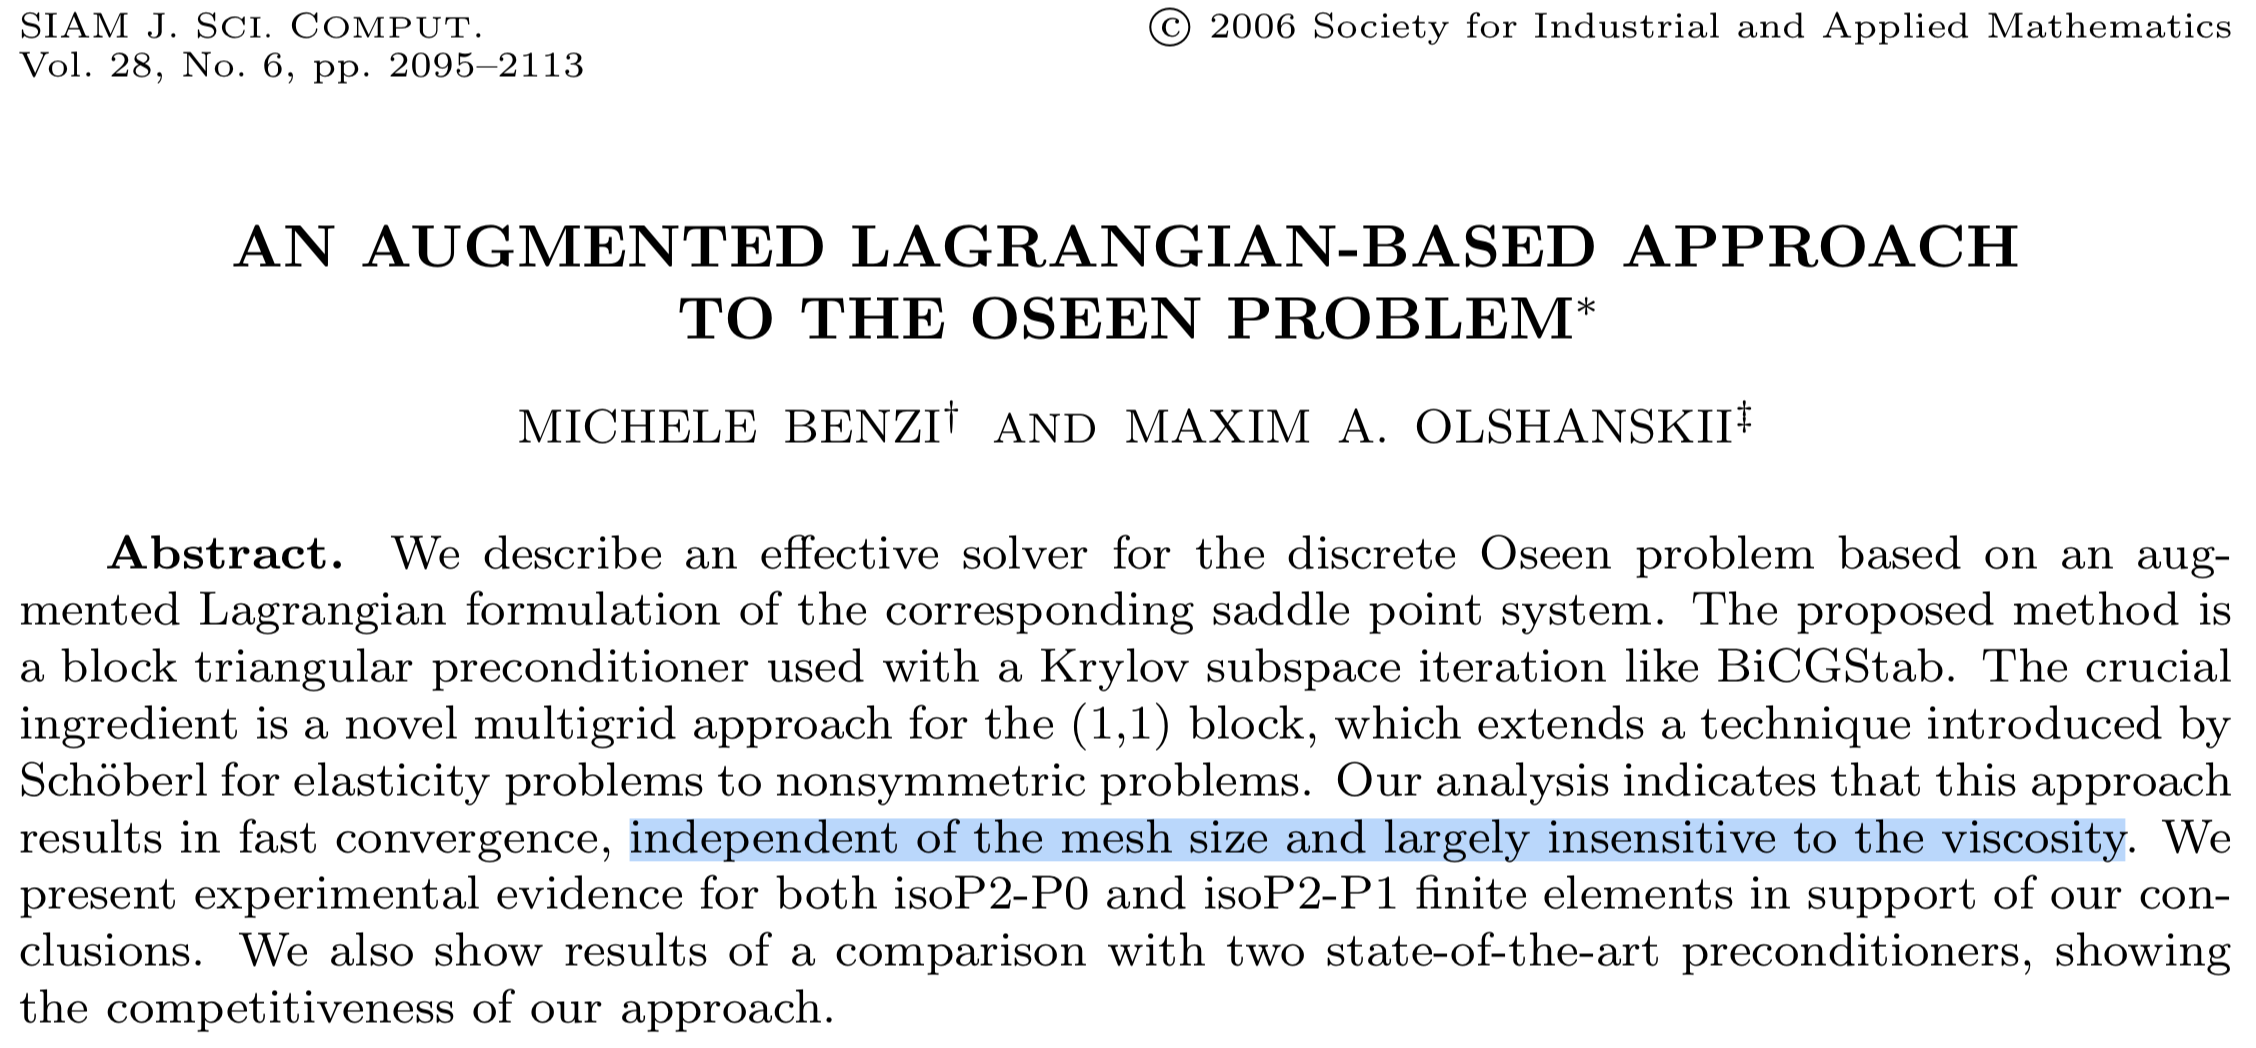
\includegraphics[width=\textwidth]{benzi06}
  \end{center}
  \pause
    \begin{block}{Observation}
    \begin{itemize}
    \item[\cmark] Reynolds-robust preconditioning
    \item[\xmark] No-one else appears to have implemented the full scheme
      (2006--2018)
    \end{itemize}
  \end{block}
\end{frame}

\begin{frame}[t]
  \frametitle{Objectives}
  \begin{itemize}
  \item Can we make the first general implementation of the method? \cmark
  \item Can we extend the solver and discretisation to three
    dimensions? \cmark
  \end{itemize}
  \pause
  \begin{block}{Three ideas}
    \begin{enumerate}
    \item Control Schur complement with an augmented Lagrangian term
    \item Kernel-capturing multigrid relaxation
    \item Robust multigrid prolongation
    \end{enumerate}
  \end{block}
  {\hfill\raggedleft\scriptsize \textcite{Farrell:2018} \arxivlink{1810.03315}{math.NA}}
\end{frame}

\begin{frame}{Augmented Lagrangian approach}
  \begin{block}{Stokes again\uncover<2->{, with augmented Lagrangian term}}
    \begin{equation*}
      \begin{aligned}
        & \underset{u\in V}{\text{minimise}} & & \int \nabla : \nabla \dx
        - \int f \cdot v \dx \uncover<2->{+ \gamma \int (\nabla \cdot
          v)^2 \dx}\\
        &\text{ subject to } & & \nabla \cdot v = 0
      \end{aligned}
    \end{equation*}
  \end{block}

  \pause
  \pause Doesn't change solution, since $\nabla \cdot v = 0$.

  \begin{theorem}[Hestenes, Fortin, Glowinski, Olshanksii, \dots]
    As $\gamma \to \infty$, the Schur complement is well
    approximated by $S^{-1} \sim -(1 + \gamma)M_p^{-1}$.
  \end{theorem}
\end{frame}

\begin{frame}
  \frametitle{\dots or discretely}
  \begin{block}{Discrete augmented Lagrangian}
    \begin{equation*}
      \begin{pmatrix}
        A + \gamma B^T M_p^{-1} B & B^T \\
        B & 0
      \end{pmatrix}
      \begin{pmatrix}
        u \\ p
      \end{pmatrix}
      =
      \begin{pmatrix}
        b \\ 0
      \end{pmatrix}
    \end{equation*}
  \end{block}

  \pause  Doesn't change solution, since $B u = 0$

  \begin{block}{New Schur complement}
    \begin{equation*}
      \hat{S}^{-1} = S^{-1} - \gamma M_p^{-1}
    \end{equation*}

    Again, as $\gamma \to \infty$, the Schur complement is well
    approximated by $\hat{S}^{-1} \sim -(1 + \gamma)M_p^{-1}$.
  \end{block}

  \pause
  \begin{center}
    These results still hold for Navier--Stokes!
  \end{center}
\end{frame}
\begin{frame}
  \frametitle{Conservation of misery}
  We now must solve either: find $u \in V \subseteq \honev$ such that
  \begin{block}{Continuous stabilisation}
    \begin{equation*}
      \nu (\nabla u, \nabla v) + (\advect{u}{w}, v) + (\advect{w}{u}, v) 
      + \gamma(\nabla \cdot u, \nabla \cdot v) = (f, v)
    \end{equation*}
  \end{block}
  \vspace{-0.5\baselineskip}
  or 
  \begin{block}{Discrete stabilisation}
    \begin{equation*}
      \nu (\nabla u, \nabla v) + (\advect{u}{w}, v) + (\advect{w}{u}, v) 
      + \gamma(\overline{\nabla \cdot u}, \overline{\nabla \cdot v}) = (f, v)
  \end{equation*}
  \end{block}
  \vspace{-0.5\baselineskip}
  for all $v \in V$, where $\overline{x}$ is the $L^2$ projection onto
  the discrete pressure space.
\end{frame}

\begin{frame}
  \frametitle{Conservation of misery II}
  \begin{exampleblock}{Good news}
    The Schur complement becomes easy to approximate as $\gamma \to \infty$.
  \end{exampleblock}
  \pause
  \begin{challenge}{Bad news}
    Our usual multigrid approaches for $\tilde{A}^{-1}$ no longer
    work for $A_\gamma := A + \gamma B^TM_p^{-1}B$, and get \emph{worse} as $\gamma \to \infty$
  \end{challenge}
  \pause
  \begin{center}
    \begin{tabular}{l| c |c}
      \toprule
      &  LU for $A_\gamma^{-1}$ & AMG for $A_\gamma^{-1}$\\
      \midrule
      $\gamma=10^{-1}$ & 15 &18\\
      $\gamma=1$ & 6 &40\\
      $\gamma=10^{1}$ & 3 &107\\
      \bottomrule
    \end{tabular}
  \end{center}
  \pause
  \begin{answer}{Goal}
    Find a $\gamma$-robust multigrid method for $A_\gamma^{-1}$.
  \end{answer}
\end{frame}

\section{Robust multigrid}

\begin{frame}
  \frametitle{Stokes case}
  \begin{itemize}
  \item Ignorning advection, then the top-left block corresponds to
    discretisation of
    \begin{equation*}
      a_{\gamma}(u, v) = \xunderbrace{\int_\Omega \nu \nabla u  : \nabla v \dx}_{\text{sym.~pos.~def.}} \quad +  \quad \textcolor{red}{\xunderbrace{\int_\Omega \gamma\div(u)\div(v) \dx}_{\text{sym.~pos.~semi-def.}}}
    \end{equation*}
    \pause
  \item The semi-definite term is singular on all solenoidal fields
    $\Rightarrow$ the system becomes \emph{nearly singular} as $\gamma
    \to \infty$
    \pause
  \item To build a $\gamma$-robust scheme we need
    \parencite{Schoeberl:1999}
    \begin{itemize}
    \item a $\gamma$-robust smoother;
    \item a prolongation operator with $\gamma$-independent continuity constant.
    \end{itemize}
  \end{itemize}
\end{frame}

\begin{frame}[t]
  \frametitle{Idea: kernel-capturing relaxation}
  Consider the problem: for $\alpha, \beta \in \mathbb{R}$, find $u \in V$ such that
  \begin{equation*}
    \alpha a(u, v) + \beta b(u, v) = (f, v) \quad \forall v \in V,
  \end{equation*}
  where $a$ is SPD, and $b$ is symmetric positive semidefinite.

  \begin{block}{Relaxation method}
    Choose a subspace decomposition
    \begin{equation*}
      V = \sum_i V_i,
    \end{equation*}
    solve the problem on each subspace and combine the updates.
  \end{block}
  \begin{exampleblock}{Example}
    If each $V_i$ is the span of a single basis function, this defines a
    Jacobi (Gauss-Seidel) iteration.
  \end{exampleblock}
\end{frame}

\begin{frame}[t]
  \frametitle{Idea: kernel-capturing relaxation}
  Define the kernel as
  \begin{equation*}
      \mathcal{N} := \{ u \in V : b(u, v) = 0 \,\, \forall v \in V \}.
  \end{equation*}
  \begin{theorem}[Sch\"oberl (1999); Lee, Wu, Xu,
    Zikatanov (2007)]
    An additive subspace correction method using subspaces $\{V_i\}$
    is parameter robust if every $u \in \mathcal{N}$ can be written as
    a sum $u = \sum_i u_i$ with $u_i \in V_i \cap \mathcal{N}$, i.e.
    \begin{equation*}
      \mathcal{N} = \sum_i \mathcal{N} \cap V_i.
    \end{equation*}
    ``The subspace decomposition \emph{captures the kernel}.''
    \nocite{Ewing:1992,Schoeberl:1999,Lee:2007}
  \end{theorem}
\end{frame}

\begin{frame}{Relaxation}
  In 2D we consider $P_2-P_0$ elements. For these one can show that \emph{star} patches 
  \begin{figure}
    \begin{center}
      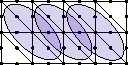
\includegraphics[width=8cm]{star}
    \end{center}
  \end{figure}
  satisfy the kernel decomposition property.
\end{frame}

\begin{frame}
  \frametitle{Idea: robust prolongation}
  \begin{theorem}[Sch\"oberl (1999)]
    Let the prolongation $P : V_H \to V_h$. A robust multigrid cycle
    requires
    \begin{equation*}
      \nu\|\nabla P u_H\|_{L^2}^2 + \gamma\|\overline{\nabla\cdot P
        u_H}\|_{L^2}^{2} \le C(\nu\|\nabla u_H\|_{L^2}^2 + \gamma\|\overline{\nabla\cdot u_H}\|_{L^2}^2)
    \end{equation*}
    with $C$ independent of both $\nu$ and $\gamma$.
  \end{theorem}
  \pause
  \begin{exampleblock}{Observation}
    Notice that if $\nabla \cdot u_H = 0$ then we have
    \begin{equation*}
      \nu\|\nabla P u_H\|_{L^2}^2 + \textcolor{red}{\gamma\|\overline{\nabla\cdot P u_H}\|_{L^2}^{2}} \le C\nu\|\nabla u_H\|_{L^2}^2
    \end{equation*}
    
    $\Rightarrow$ we need $P$ to map coarse-grid div-free fields to
    (nearly) div-free fields on the fine grid.
  \end{exampleblock}
\end{frame}

\begin{frame}
  \frametitle{Robust prolongation: 2D}
  \begin{itemize}
  \item<1-> Discrete divergence $\Leftrightarrow$ flux across facets
  \item<1-> $V_h \subset V_h \implies$ flux across coarse-grid faces is
    preserved.
  \item<2-> $P_2-P_0$ not a \emph{divergence-free} discretisation
    $\Rightarrow$ solve a local Stokes problem to \emph{fix} the flux
    on new facets.
  \end{itemize}
  \begin{center}
    \only<1>{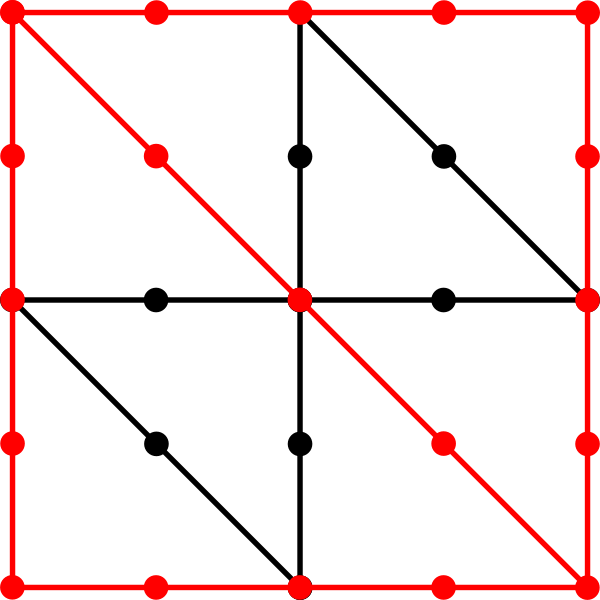
\includegraphics[height=0.4\textheight]{prolongation_nopatch}}
    \only<2->{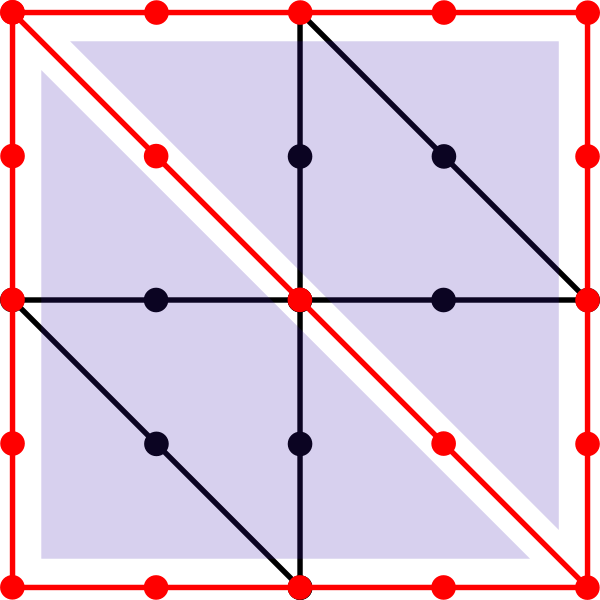
\includegraphics[height=0.4\textheight]{prolongation}}
  \end{center}
\end{frame}

\begin{frame}
  \frametitle{What about 3D}
  \begin{overlayarea}{\textwidth}{0.7\textheight}
    Which element should we choose?

    \begin{tabular}{lccc}
      & \only<1->{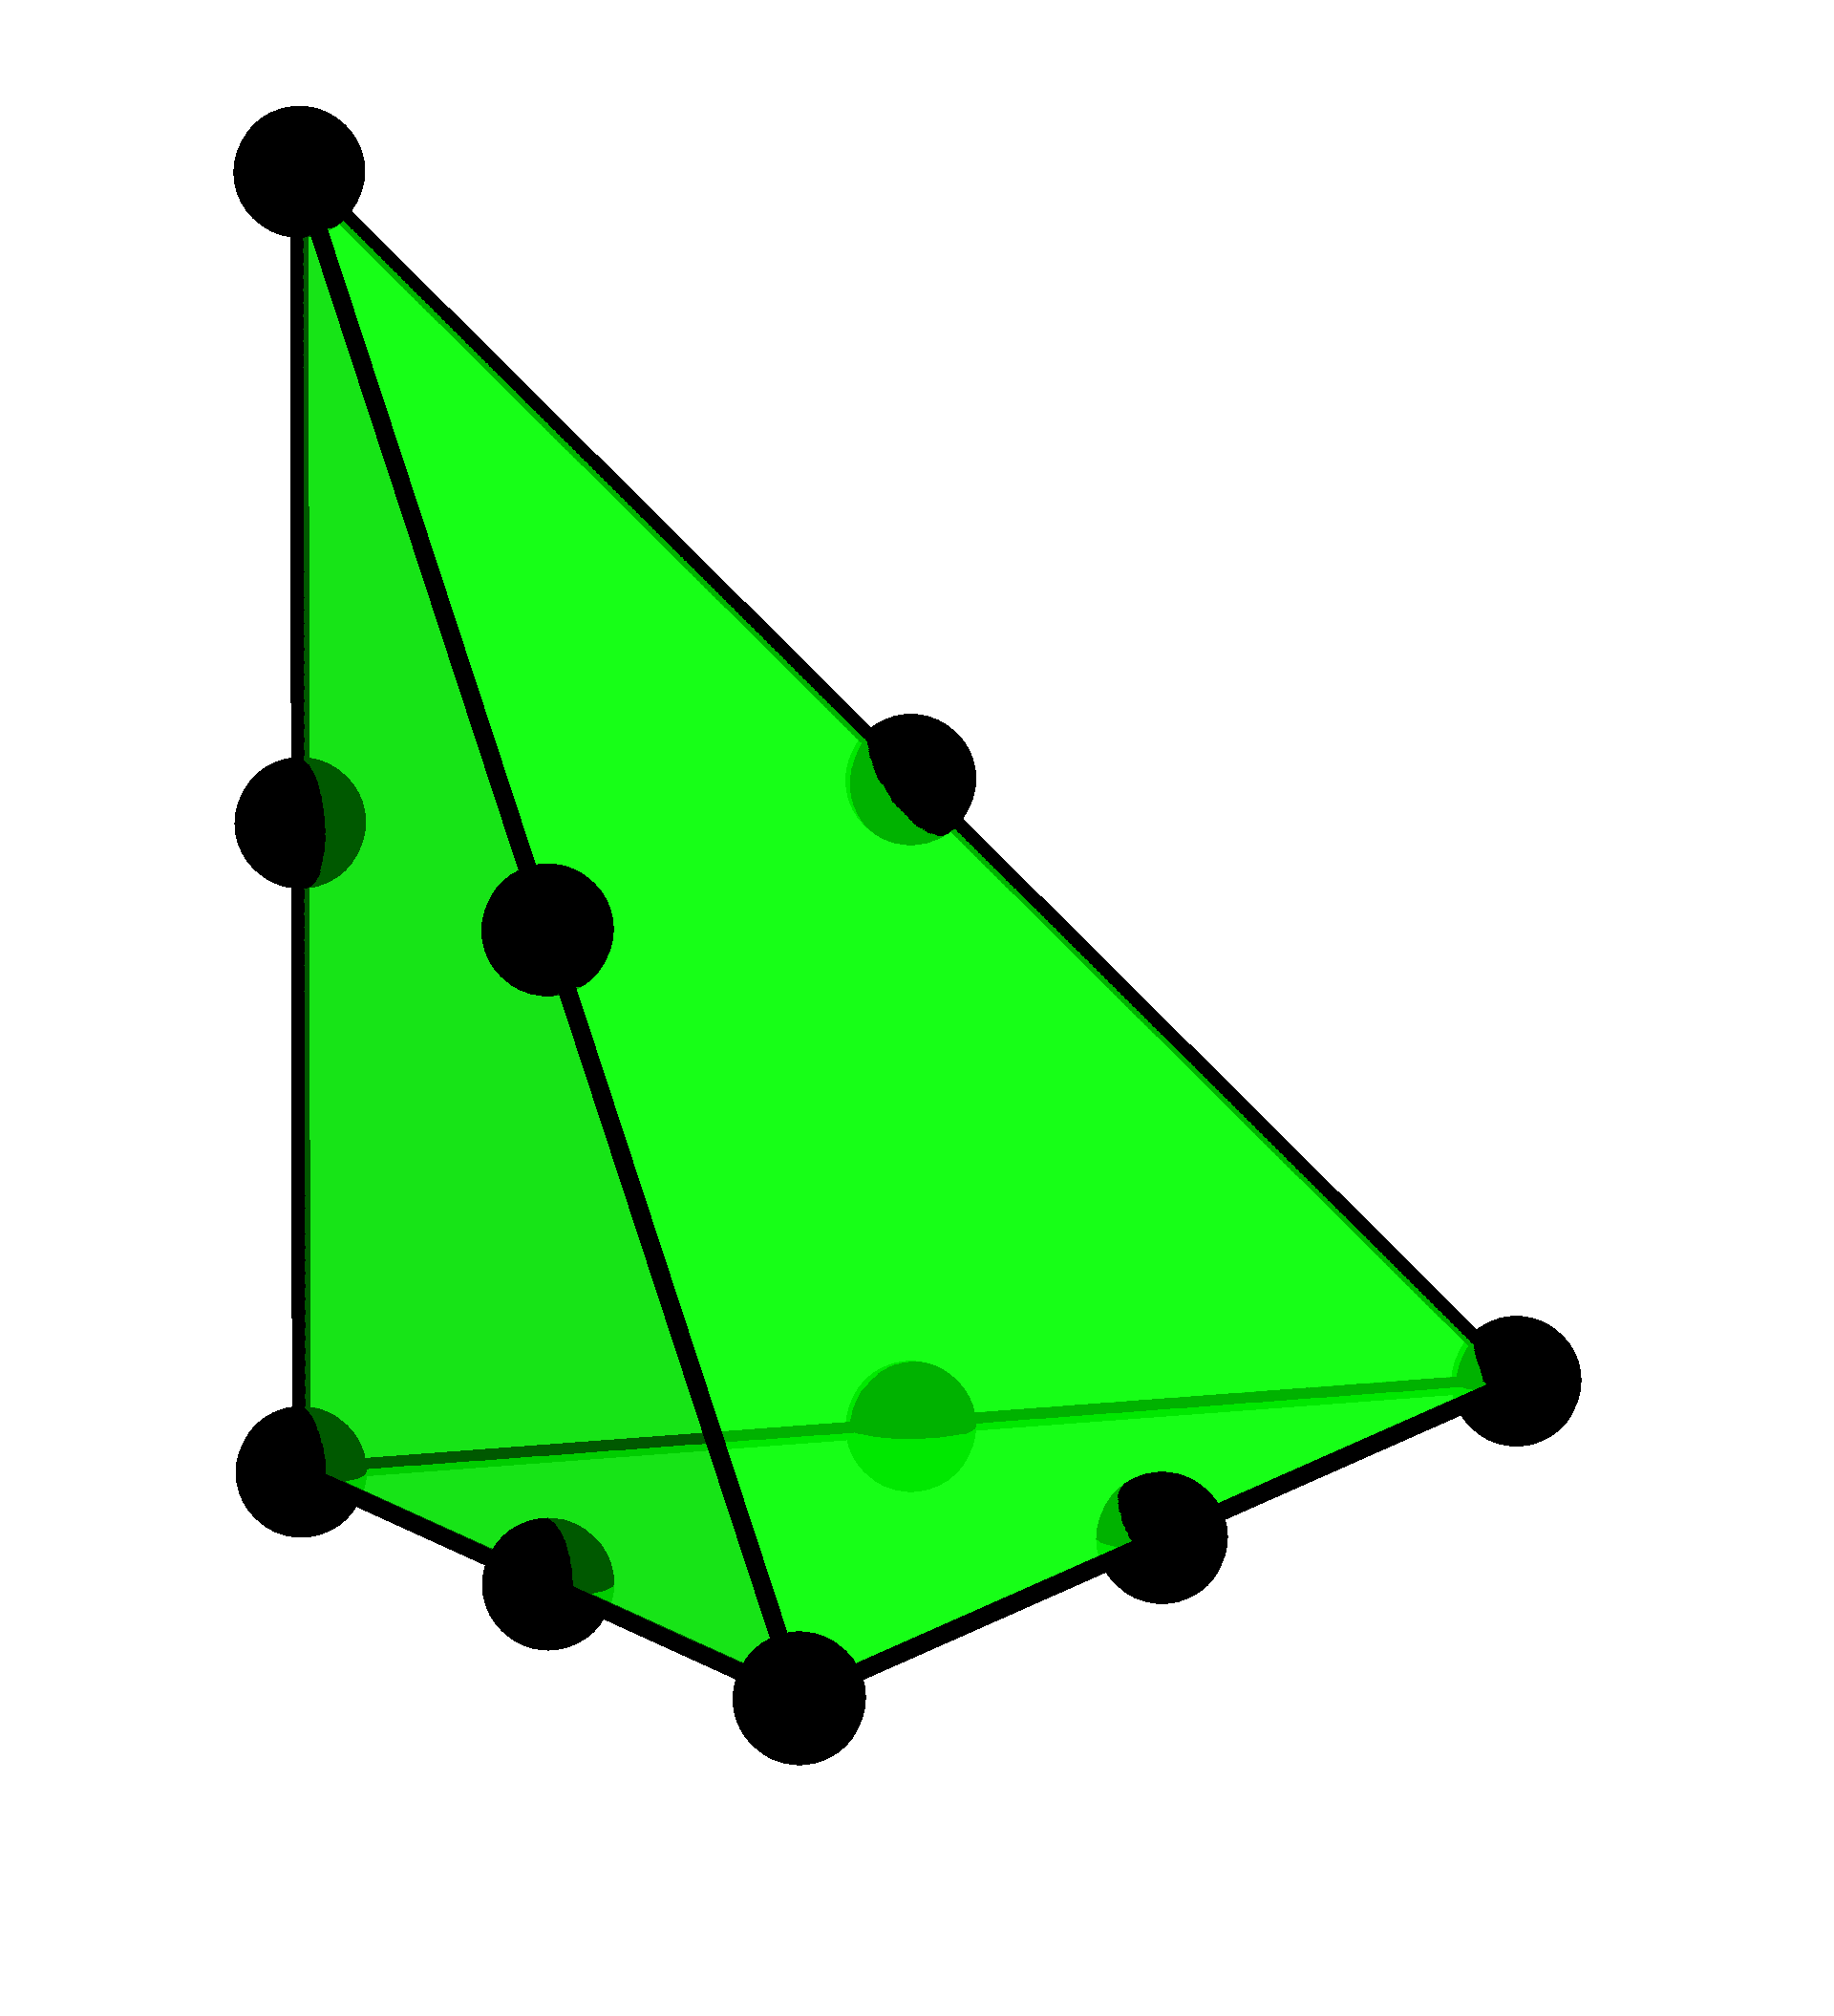
\includegraphics[width=0.3\textwidth]{P2}} & \only<3->{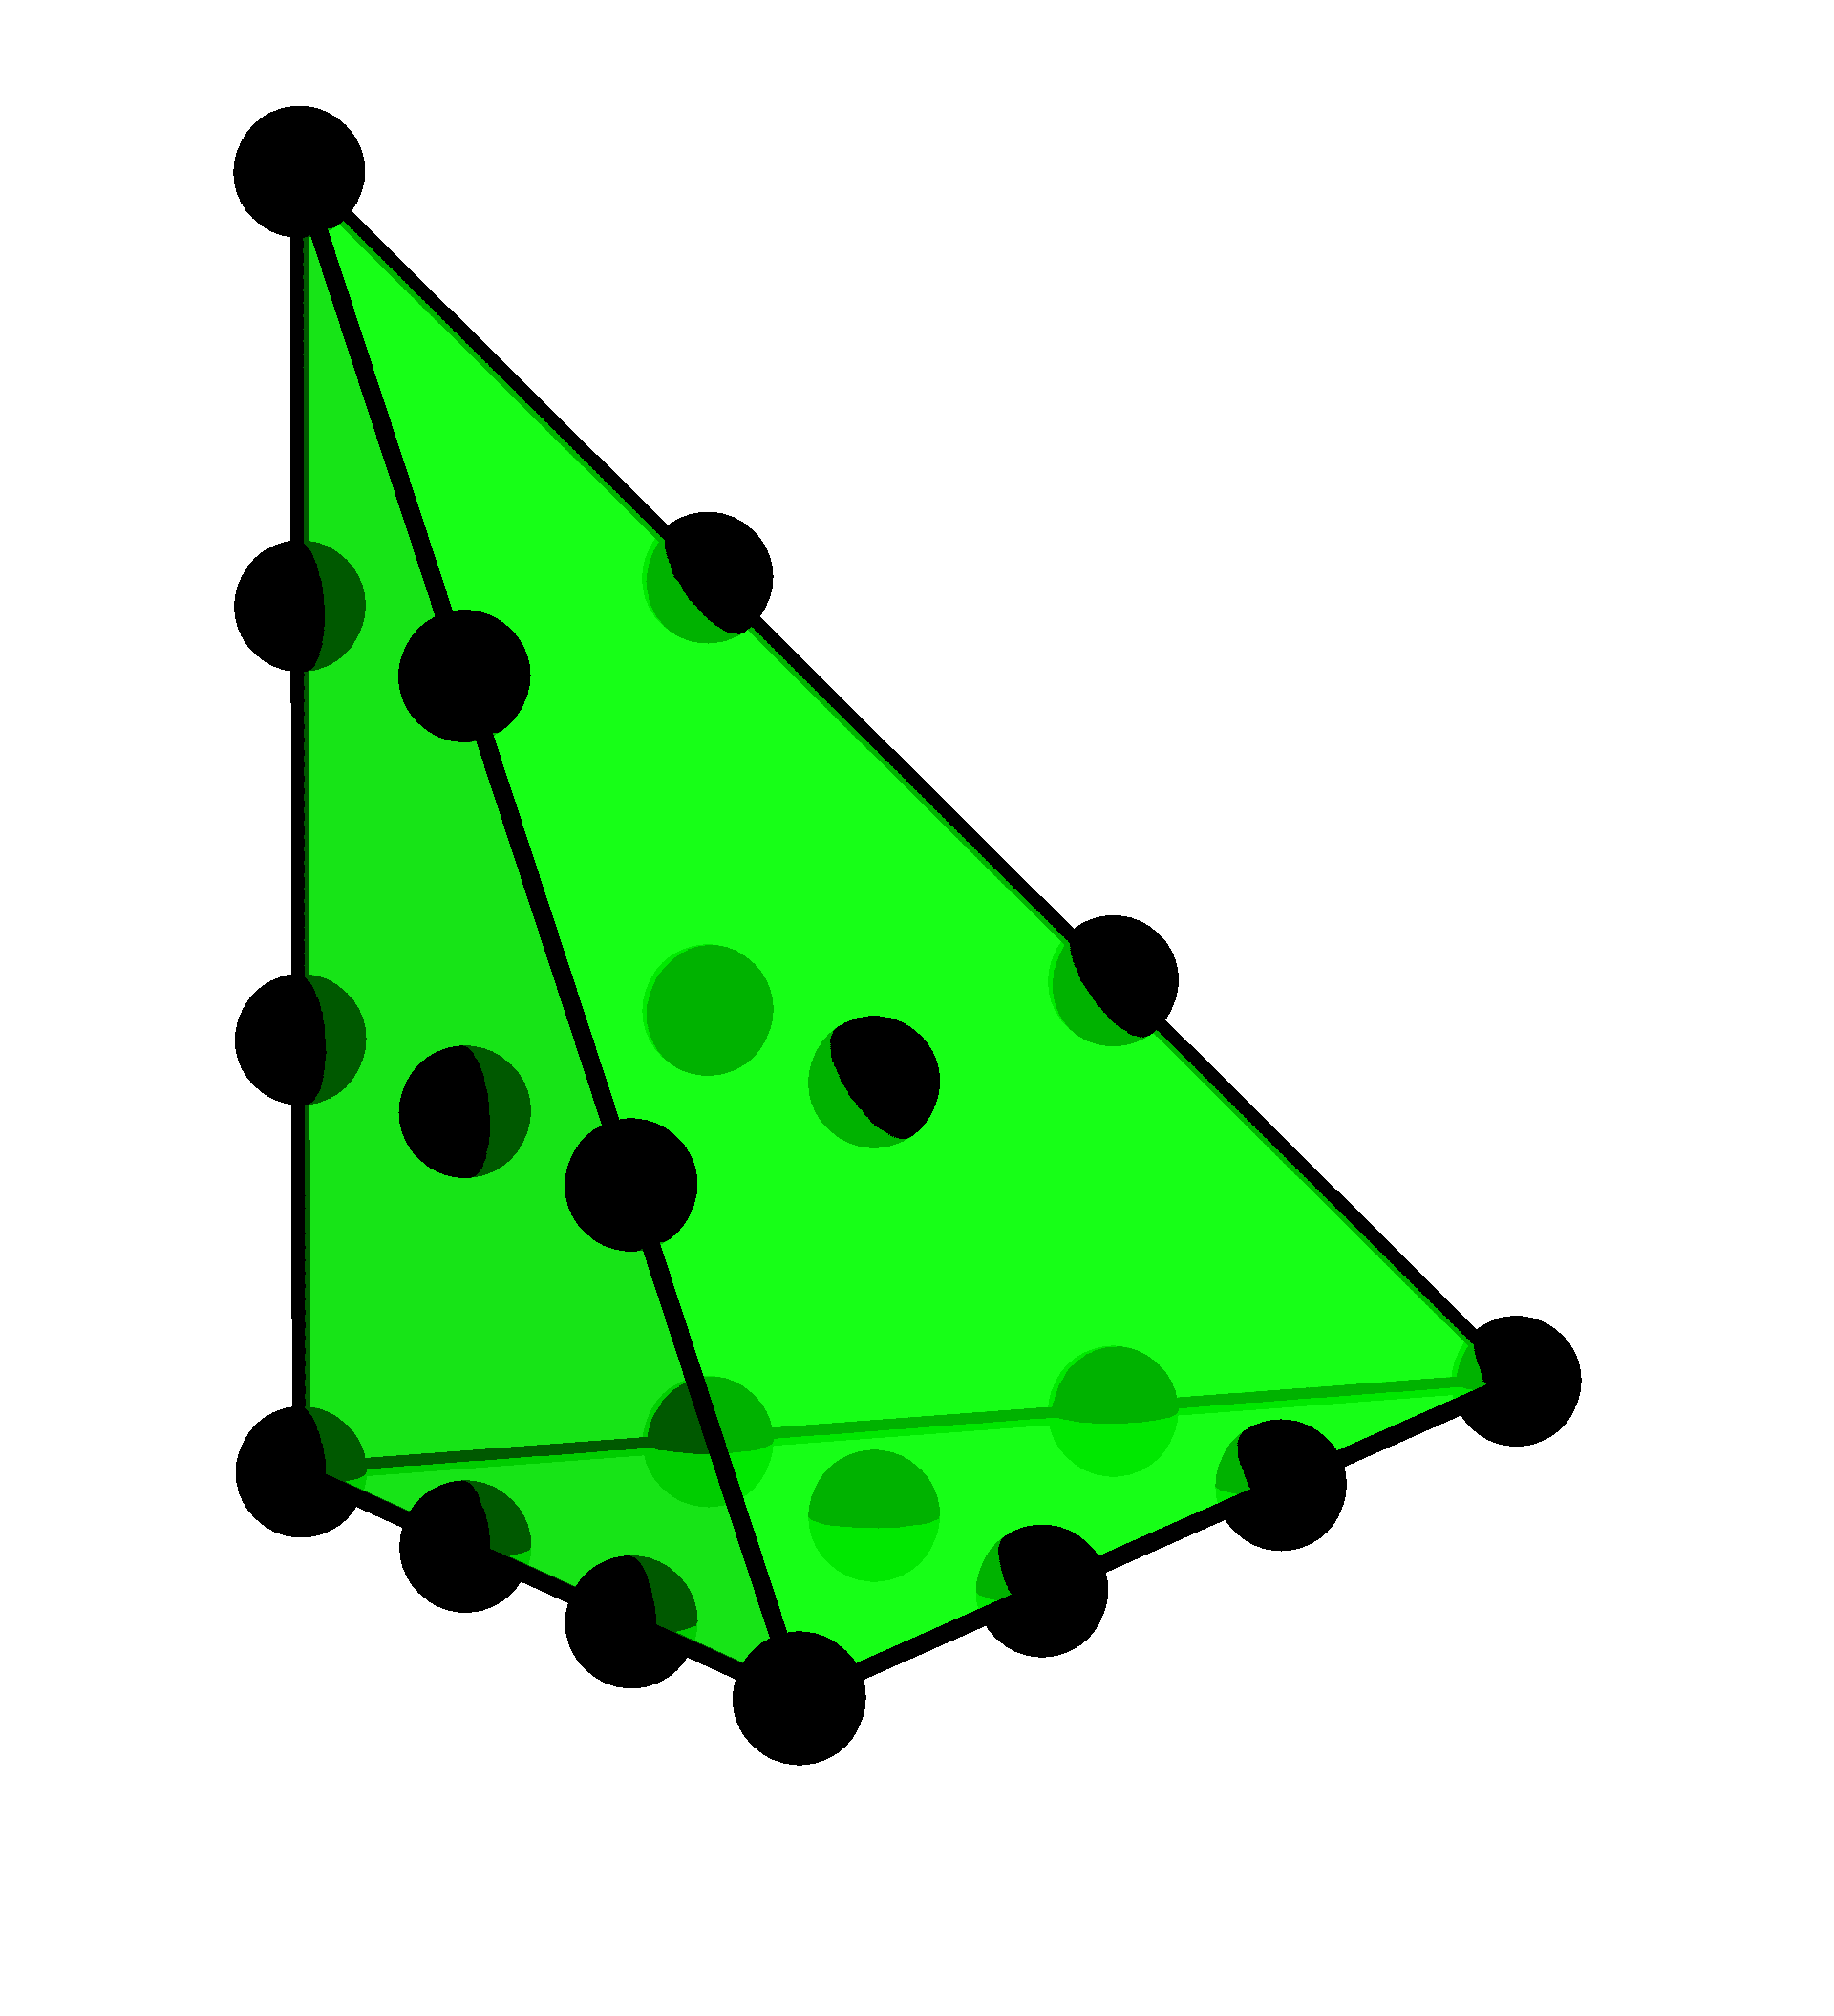
\includegraphics[width=0.3\textwidth]{P3}} & \only<4->{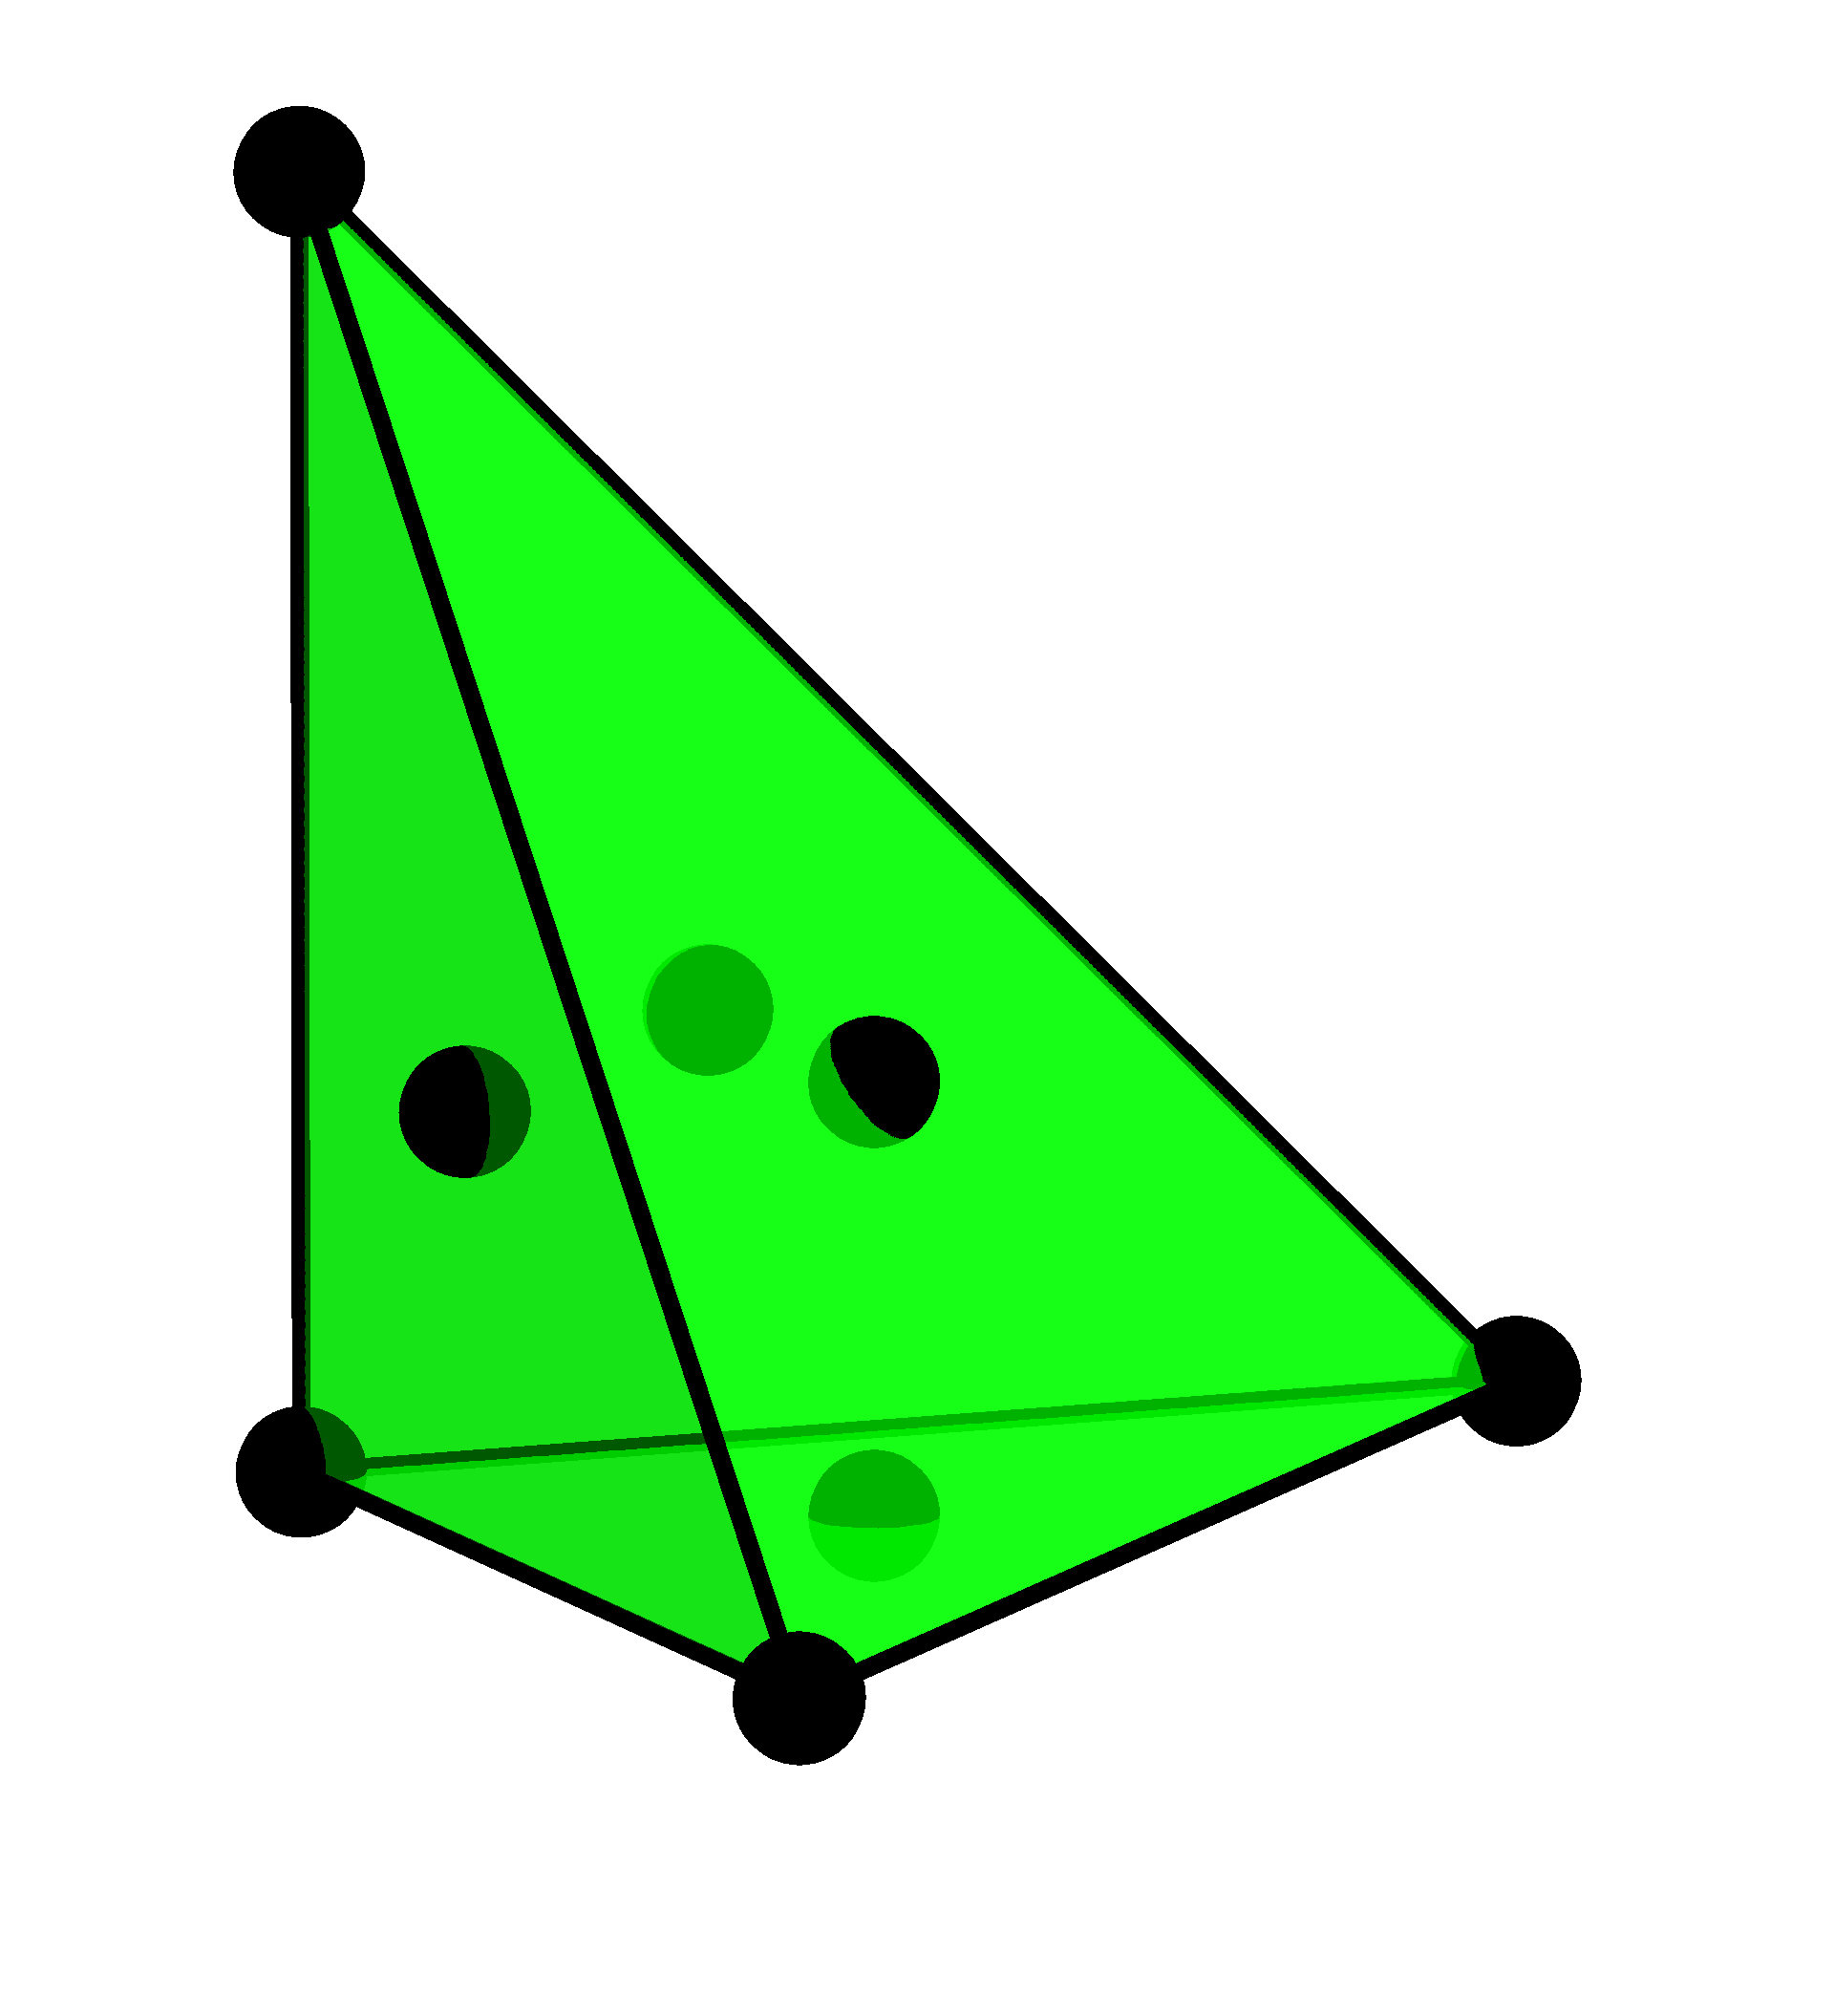
\includegraphics[width=0.3\textwidth]{P1FB}} \\
      \hspace{-0.5cm}
      & \uncover<1->{ $P_2$}\quad\ ~ & \uncover<3->{ $P_3$}\ \ ~ & \uncover<4->{ $P_1 \oplus \text{FB}$}\ ~\\
      \hspace{-0.5cm}
      stable & \uncover<2->{\xmark}\quad\ ~ & \uncover<3->{\cmark}\ \ ~ & \uncover<4->{\cmark}\ \ ~
    \end{tabular}
  \end{overlayarea}
\end{frame}

\begin{frame}{Prolongation --- 3D}
  Problem: $V_H\not\subset V_h$
  \begin{center}
    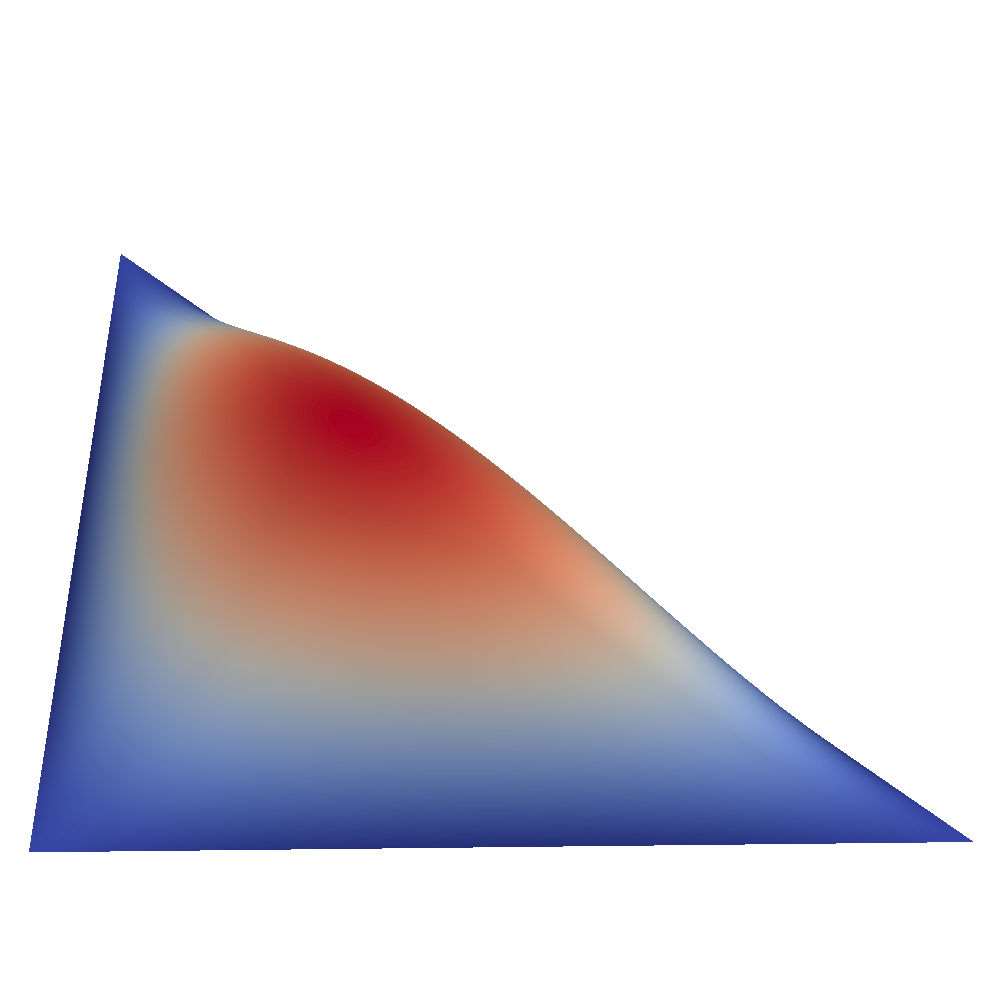
\includegraphics[width=0.3\textwidth]{bubble}
    \qquad
    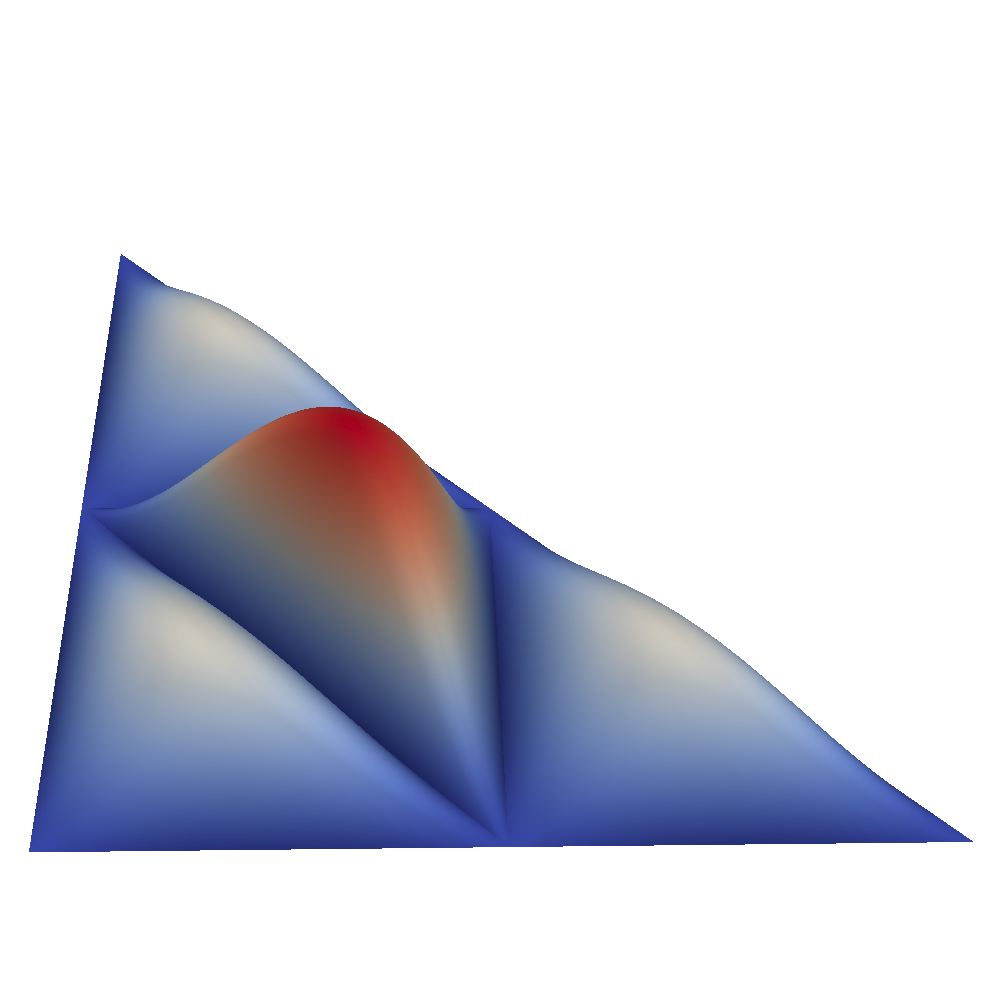
\includegraphics[width=0.3\textwidth]{bubble_prolong}
  \end{center}
  Solution:
  \begin{enumerate}
  \item Split into $P_1$ and facet bubble part, prolong the two parts separately.
  \item Scale the facet bubble components to preserve flux across coarse grid facets.
  \item Solve local Stokes problem to fix divergence inside coarse cell.
  \end{enumerate}
\end{frame}

\section{Numerical results}

\begin{frame}{Full solver}
   \begin{center}
       \resizebox{\textwidth}{!}{
   \begin{tikzpicture}[%
  every node/.style={draw=black, thick, anchor=west},
  grow via three points={one child at (0.0,-0.7) and
  two children at (0.0,-0.7) and (0.0,-1.4)},
  edge from parent path={(\tikzparentnode.210) |- (\tikzchildnode.west)}]
  \node {Continuation}
    child { node {Newton solver with line search}
      child { node {Krylov solver (FGMRES)}
        child { node {Block preconditioner}
          child { node {Approximate Schur complement inverse}}
          child { node {F-cycle on augmented momentum block}
              child { node {Coarse grid solver}
                child { node {LU factorization on assembled matrix}}
              }
              child [missing] {}
              child { node {Prolongation operator}
                child { node {Local solves over coarse cells}}
              }
              child [missing] {}
              child { node {Relaxation}
                child { node {GMRES}
                  child { node {Overlapping additive Schwarz iteration}}
                }
              }
          }
        }
      }
    };
\end{tikzpicture}}
   \end{center} 
\end{frame}

\begin{frame}
  \frametitle{Numerical results --- 2D}
  \begin{table}[htbp]
    \centering
    \begin{tabular}{cc|ccccc}
      \toprule
      \# ref. & \# dofs & \multicolumn{5}{c}{Reynolds number} \\
              && 10 & 100 & 1000 &  5000 & 10000\\
      \midrule
      \multicolumn{7}{c}{Lid Driven Cavity}\\
      \midrule
      1 & $1.0 \times 10^4$ & 3.00 &  4.00 &  5.33 & 8.50 & 11.0 \\
      2 & $4.1 \times 10^4$ & 2.50 &  3.67 &  6.00 & 8.00 & 9.50 \\
      3 & $1.6 \times 10^5$ & 2.50 &  3.00 &  5.67 & 7.50 & 9.00 \\
      4 & $6.6 \times 10^5$ & 2.50 &  3.00 &  5.00 & 7.00 & 8.00 \\
      \midrule
      \multicolumn{7}{c}{Backwards Facing Step}\\
      \midrule
      1 & $1.1 \times 10^6$ & 2.33 & 3.75 & 4.50 & 4.50 & 8.00\\
      2 & $4.5 \times 10^6$ & 3.00 & 3.25 & 4.50 & 4.50 & 5.50\\
      3 & $1.8 \times 10^7$ & 3.00 & 5.75 & 4.00 & 4.00 & 6.00\\
      \bottomrule
    \end{tabular}
    \caption{Average number of outer Krylov iterations per Newton step for two 2D benchmark problems.}
  \end{table}
\end{frame}

\begin{frame}
  \frametitle{Numerical results --- 3D}
  \begin{table}[htbp]
    \centering
    \begin{tabular}{cc|ccccc}
      \toprule
      \# ref. & \# dofs & \multicolumn{5}{c}{Reynolds number} \\
              && 10 & 100 & 1000 & 2500 & 5000 \\
      \midrule
      \multicolumn{7}{c}{Lid Driven Cavity}\\
      \midrule
      1 & $2.1 \times 10^6$ & 4.50 & 4.00 & 5.00 & 4.50 & 4.00 \\
      2 & $1.7 \times 10^7$ & 4.50 & 4.33 & 4.50 & 4.00 & 4.00 \\
      3 & $1.3 \times 10^8$ & 4.50 & 4.33 & 4.00 & 3.50 & 7.00 \\
      4 & $1.1 \times 10^9$ & 4.50 & 3.66 & 3.00 & 5.00 & 5.00 \\
      \midrule
      \multicolumn{7}{c}{Backwards facing step}\\
      \midrule
      1 & $2.1 \times 10^6$ & 4.50 & 4.00 & 4.00 & 4.50 & 7.50  \\
      2 & $1.7 \times 10^7$ & 5.00 & 4.00 & 3.33 & 4.00 & 10.00 \\
      3 & $1.3 \times 10^8$ & 6.50 & 4.50 & 3.50 & 3.00 & 8.00  \\
      4 & $1.0 \times 10^9$ & 7.50 & 3.50 & 2.50 & 3.00 & 6.00  \\
    \end{tabular}
    \caption{Average number of outer Krylov iterations per Newton step for two 3D benchmark problems.}
    \label{tab:ourldc3d}
  \end{table}
\end{frame}

\begin{frame}[t]
  \frametitle{Computational performance --- 3D}
  \pgfplotstableread[col sep=comma, row sep=\\]{%
    Cores,Time,Dofs\\
    48,5.3e1,2134839\\
    384,6.9e1,16936779\\
    3072,6.1e1,134930451\\
    24576,6.6e1,1077196323\\
  }\ldctable
  % [55.02509561666667, 68.57286605, 57.029964033333336, 69.39903468333333]
  \pgfplotstableread[col sep=comma, row sep=\\]{%
    Cores,Time,Dofs\\
    48,5.5e1,2107839\\
    384,6.9e1,16534263\\
    3072,5.7e1,130973115\\
    24576,6.9e1,1042606515\\
  }\bfstable
  % [53.140734383333324, 68.56801668333334, 61.468243016666655, 65.64923281666665]
  \begin{columns}
    \begin{column}{0.5\textwidth}
      \begin{center}
      \begin{tikzpicture}
        \begin{semilogxaxis}[
          width=0.955\linewidth,
          height=0.9\linewidth,
          log basis x=2,
          ymin=0,
          ymax=80,
          xtick=data,
          xticklabels from table={\ldctable}{Cores},
          extra x ticks={48, 384, 3072, 24576},
          extra x tick labels={$[2.13]$, $[16.9]$,$[135]$,$[1077]$},
          extra x tick style={tick label style={yshift=-2.5ex}},
          xlabel={Cores\\{}[DoFs $\times 10^6$]},
          xlabel style={align=center, style={yshift=-0.5ex}},
          ylabel near ticks,
          ylabel style={align=center, text width=4cm},
          title={3D lid-driven cavity.},
          ylabel={Time [min]},
          ]
          \addplot+ table[x=Cores,y=Time] {\ldctable};
        \end{semilogxaxis}
      \end{tikzpicture}
    \end{center}
    \end{column}
    \begin{column}{0.5\textwidth}
      \begin{center}
      \begin{tikzpicture}
        \begin{semilogxaxis}[
          width=0.95\linewidth,
          height=0.9\linewidth,
          log basis x=2,
          ymin=0,
          ymax=80,
          xtick=data,
          xticklabels from table={\bfstable}{Cores},
          extra x ticks={48, 384, 3072, 24576},
          extra x tick labels={$[2.11]$, $[16.5]$,$[131]$,$[1043]$},
          extra x tick style={tick label style={yshift=-2.5ex}},
          xlabel={Cores\\{}[DoFs $\times 10^6$]},
          xlabel style={align=center, style={yshift=-0.5ex}},
          ylabel near ticks,
          ylabel style={align=center, text width=4cm},
          title={3D backwards-facing step.},
          ]
          \addplot+ table[x=Cores,y=Time] {\bfstable};
        \end{semilogxaxis}
      \end{tikzpicture}
    \end{center}
    \end{column}
  \end{columns}
  \begin{center}
    50 continuation steps
  \end{center}
\end{frame}

\section{Pressure robust discretisations}

\begin{frame}
  \frametitle{Why pressure robust?}
  Standard error estimate for Stokes \parencite{John:2017}
  \begin{equation*}
    \|\nabla(u - u_h)\|_{L^2} \le 2 \inf_{\tilde{u}}\|\nabla(u - \tilde{u})\|_{L^2} + \textcolor{red}{\nu^{-1} \inf_{\tilde{p}} \|p - \tilde{p}\|_{L^2}}
  \end{equation*}

  If the element pair is \emph{divergence-free} ($\nabla \cdot V_h \subset Q_h$), then this estimate can be improved to
  \begin{equation*}
    \|\nabla(u - u_h)\|_{L^2} \le 2 \inf_{\tilde{u}}\|\nabla(u - \tilde{u})\|_{L^2}    
  \end{equation*}

  Similar optimal estimates can be shown for the time-dependent problem \parencite{Linke:2019}.
\end{frame}

\begin{frame}[t]
  \frametitle{Element choices}
  \begin{overlayarea}{\textwidth}{\textheight}
    \begin{onlyenv}<1-2>
      \vspace{-\baselineskip}
      \begin{block}{$H(\div)$-conforming}
        Choose discrete element pair from the de Rham complex:
        \begin{equation*}
          \mathbb{R} \xrightarrow{\operatorname{id}} H^1 \xrightarrow{\grad} H(\curl) \xrightarrow{\curl} H(\div) \xrightarrow{\div} L^2 \xrightarrow{\operatorname{null}} 0.
        \end{equation*}
      \end{block}
      \vspace{-0.5\baselineskip}
      \begin{exampleblock}{Example}
        \textcite{Raviart:1977}
        \begin{equation*}
          V_h \times Q_h = \operatorname{RT}_k \times P_k^{\text{disc}}
        \end{equation*}
      \end{exampleblock}
      \vspace{-0.5\baselineskip}
      \uncover<2>{
        \small
        \begin{itemize}
        \item[\cmark] Nested spaces $V_H \subset V_h$: regular prolongation suffices
        \item[\cmark] Arbitrary order
        \item[\cmark] Commuting diagram $\Rightarrow$ kernel decomposition ``just works''
        \item[\xmark] Not $H^1$-conforming: need penalty or hybridised scheme for $\nabla^2$ term
        \item[\xmark] Requires more code development in PETSc
        \end{itemize}
      }
    \end{onlyenv}
    \begin{onlyenv}<3->
      \vspace{-\baselineskip}
      \begin{block}{$H^1$-conforming}
        Choose discrete element pair from the Stokes complex:
        \begin{equation*}
          \mathbb{R} \xrightarrow{\operatorname{id}} H^2 \xrightarrow{\grad} H^1(\curl) \xrightarrow{\curl} H^1 \xrightarrow{\div} L^2 \xrightarrow{\operatorname{null}} 0.
        \end{equation*}
      \end{block}
      \vspace{-0.5\baselineskip}
      \begin{exampleblock}{Example}
        \textcite{Scott:1985}
        \begin{equation*}
          V_h \times Q_h = P_{k} \times P_{k-1}^{\text{disc}}
        \end{equation*}
      \end{exampleblock}
      \vspace{-0.5\baselineskip}
      \uncover<4->{
        \small
        \begin{itemize}
        \item[\xmark] Low degree $k = d$ versions not inf-sup on all meshes
        \item[\cmark] Arbitrary order for $k$ sufficiently large
        \item[\xmark] No commuting diagram (yet)
        \item[\cmark] $H^1$-conforming
        \item[\cmark] All code already exists
        \end{itemize}
      }
    \end{onlyenv}
  \end{overlayarea}
\end{frame}

\begin{frame}
  \frametitle{Scott--Vogelius pair}
  For $k \ge d$, pair is stable on \emph{barycentrically} refined meshes.

  Build a non-nested multigrid hierarchy.

  \pause
  \begin{center}
    \begin{tikzpicture}[scale=2]
      \foreach \i in {1, 2, 3} {
        \begin{scope}[shift={($(\i*1.5-1.5, 0)$)}]
          \DrawIterated{\i}{0}{0}{1}{0}{0.5}{\fpeval{sqrt(3)/2}}
        \end{scope}
        \begin{scope}[shift={($(\i*1.5-1.5, -1.5)$)}]
          \DrawIteratedBary{\i}{0}{0}{1}{0}{0.5}{\fpeval{sqrt(3)/2}};
        \end{scope}

        \draw[-stealth, very thick] ($(-1 + 1.5*\i, -0.1)$) -- +(0, -0.4);
        \ifnum\i=3
        \relax
        \else
        \draw[-stealth, very thick] ($(-0.5 + 1.5*\i, 0.5)$) -- +(0.5, 0);
        \fi
      }
    \end{tikzpicture}
  \end{center}
\end{frame}

\begin{frame}
  \frametitle{Discrete complex --- 2D}
  \begin{center}
    \includestandalone[width=0.75\textwidth]{./../pictures/HCT-complex}
  \end{center}
  \pause
  Requires bigger patch in smoother
  \begin{center}
    \includestandalone[height=0.5\textheight]{./\jobname.figures/macrostar}
  \end{center}
\end{frame}

\begin{frame}
  \frametitle{Discrete complex --- 3D}
  \begin{itemize}
  \item Discrete exact sequence developed in \textcite{Fu:2018}, $k \ge 3$
  \item No commuting projections (yet)
  \item[$\Rightarrow$] need to work a bit harder in the theory to prove convergence of scheme
  \item In practice, same idea: ``macro patches'' work fine.
  \item[$\Rightarrow$] some new conjectures on basis for $C^1$ functions
  \end{itemize}
\end{frame}

\begin{frame}
  \frametitle{Conclusions \& outlook}
  \begin{exampleblock}{Main result}
    It is possible to solve the Navier--Stokes equations in a Reynolds-robust way!

    Even for exactly divergence-free discretisations
  \end{exampleblock}

  \pause
  \begin{answer}{Ongoing work}
    Large-scale runs for Scott-Vogelius element pair.

    Tidying up proof of convergence.
  \end{answer}

  \pause
  \begin{challenge}{Other discretisations}
    \begin{itemize}
    \item Scott-Vogelius rather expensive. A lot of interest in
      $H(\div)$-conforming, and hybridised $H(\div)$-conforming
      methods.
    
    \item Can we do this on general non-nested meshes?
      
    \item[$\Rightarrow$] needs divergence-preserving prolongation: Fortin operators?
  \end{itemize}
  \end{challenge}
\end{frame}
\appendix

\begin{frame}[t,allowframebreaks]
  \frametitle{References}
  \printbibliography[heading=none]
\end{frame}

\end{document}
